\chapter{Methodology and Demonstration}
\label{ch:demo_method}

This chapter first covers the methodology of the proposed work by introducing
each experimental component in Section \ref{sec:expmeth}. Section
\ref{sec:training} discusses how the training data is simulated for input to
the machine learning algorithms.  Section \ref{sec:statmodel} is about how
these will use the features and labels of the training data to statistically
formulate a model for prediction of a new instance, which has only features and
no label.  The algorithms will be evaluated for accuracy and validated, as
shown in Section \ref{sec:valid}.

Next is the demonstration of these experimental components, by first showing in
Section \ref{sec:results} how the initial results guided the next steps for
future experiments, discussed in Section \ref{sec:newtrain}.  Steps taken
towards model comparison (or even comparison against non-statistical methods)
are shown in \ref{sec:compare}.\todo{update me if necessary}

\section{Experimental Methodology}
\label{sec:expmeth}

This work incorporates some methods and suggestions from previous work on the
subject \cite{dayman_feasibility_2013} regarding machine learning model
performance with respect to information reduction, and expands upon it in two
ways. The first is adding a different information reduction technique via
applying a gamma spectroscopy \gls{DRF} to the \gls{SNF} nuclide recipes, which
can calculate various spectra based on the types of gamma detectors available
to the forensics community.  Secondly, a more advanced machine learning
algorithm, support vector regression, is included so as to compare more complex
models against the simpler models.  A schematic of the workflow involving
the experimental components is shown here in Figure \ref{fig:method}.  This
section covers each of them as follows.

\begin{figure}[!htb]
  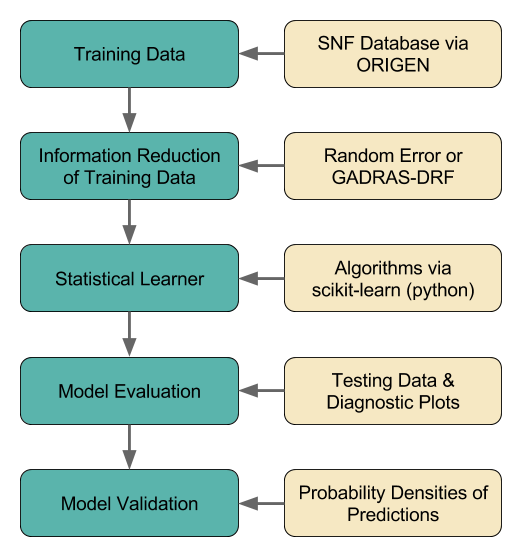
\includegraphics[width=0.9\linewidth]{./chapters/demo_method/methodology.png}
  \caption{Methodology of the proposed experiment.}
  \label{fig:method}
\end{figure}

After the initial training data is simulated in Section \ref{sec:snfsim}, with
a possible information reduction step in Section \ref{sec:inforeduc}, it will
be input to a statistical learner. While algorithm choice is discussed in
Section \ref{sec:choice}, the main goal for these machine-learned models is to
predict reactor parameters associated with some unknown \gls{SNF}. This is
shown in Section \ref{sec:rxtrparam}. To both understand the performance and
validate the models, the results are then evaluated for over- or under-fitting,
which is in Section \ref{sec:algeval}.  But validation is more than just making
sure the models are properly fit to the data.  Perhaps the training set was not
representative of the actual data space, whereas other methods do not rely on
the data space for results. So, lastly, comparison against other algorithms as
well as other methods is described in Section \ref{sec:algcompare}.

\subsection{Training Data}
\label{sec:training}
\begin{figure}[H]
  \centering
  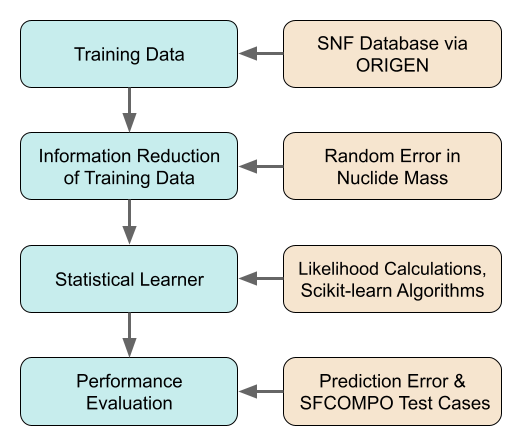
\includegraphics[width=0.7\linewidth]{./chapters/exp1/methodology1.png}
  \caption{First portion of the flowchart from Figure \ref{fig:method} being 
           described in this section.}
\end{figure}

Of interest to an entity trying to create a weapon is partially irradiated fuel
if they have plutonium separations capabilities or any radioactive substance in
the case of a dirty bomb. Thus, this work focuses on \gls{SNF} from commercial
power reactors. Ideally, a large enough database of \gls{SNF} nuclide assays
would be able to be used for this work. Since that does not exist, the 
database will be simulated via \gls{ORIGEN-ARP} \cite{origen, origenarp}.  

\subsection{Simulation Fidelity}
\label{sec:fidelity}

Nuclear fuel cycle studies involve tracking the material flow of nuclear fuel.
This can be anywhere from mining to waste management, or focus on a process
step in between. Fuel cycle studies are not necessarily nuclear-specific. For
example, they can be used to evaluate economic predictions, environmental
impact, transportation planning, etc.  In order to draw conclusions from these
studies, it is common to use a nuclear fuel cycle simulator that tracks the
quantities of interest. These allow the comparison of different fuel types,
reactor technologies, material processing steps, etc. 

There are simplifications researchers need to make in order to experiment in a
controlled way. Fuel cycle simulators, built for a specific needs, must remove
complicating factors that are less relevant to the study.  For example, one
tool might be suited well to large-scale systems analysis with little nuclear
physics included in the models, and another might focus on detailed isotopics
within a system to track plutonium.

Because a large portion of a nuclear forensics investigation relies on
measuring isotopics, this work used \gls{ORIGEN} \cite{origen}, which is a part
of the \gls{SCALE} 6.2 modeling and simulation suite of computational tools
developed for nuclear design and safety \cite{scale}. \gls{ORIGEN} was chosen
for its physically detailed models of activation, depletion, and decay.
Specifically, the ARP module of the code was used: \gls{ORIGEN-ARP}
\cite{origenarp}.

\gls{ORIGEN} calculates time-dependent nuclide concentrations (or quantities
derived from these) that result from activation and depletion calculations. The
physics (i.e., neutron transport and decay) calculations are carried out in
other \gls{SCALE} modules that solve the depletion equations.  This generates
libraries for \gls{ORIGEN} that include the probabilities of reaction (i.e.,
cross sections) for the system.

To obtain an \gls{SNF} recipe from a reactor simulation, \gls{ORIGEN} uses the
desired input power generation with the cross section library to calculate a
flux, the resulting depletion, and the end composition (i.e., isotopic recipes
or nuclide vectors).  Another output is decay; the composition is computed
using decay equations with nuclear data \cite{endf}. These compositions provide
source terms for other calculations, such as decay emission spectra from
neutrons, alpha particles, beta particles, and gamma rays. Other derived
quantities like activity, decay heat, or radiological hazard factors are also
an option.

\gls{ORIGEN-ARP} allows users to access a wider range of simulations by
interpolating between the pre-calculated libraries instead of creating new
libraries.  It is known to be validated for \gls{LWR} \gls{SNF}
\cite{lwr_valid}. Additionally, recycled \gls{SNF} in the form of mixed oxide
fuel has been benchmarked for the relevant reactors \cite{mox_valid}.  Through
\gls{ORIGEN}, given an initial material composition, some reactor operation
parameters, and a reactor type, one can quickly perform many different nuclear
reactor simulations and obtain \gls{SNF} recipes.

\todo[inline]{This section needs more information about ORIGEN-ARP validation
and maybe some nuclides that are known to perform poorly from ARP sims. Can
show a generic example from one of my sources, and or an example of trying to
match an ORIGEN-ARP simulation to an SFCOMPO entry. It is important to inform
that this training set as ground truth is not perfect truth, for some nuclides
more than others. The goal is to explain the ARP validation without getting
too deep.  This tool was necessary for the 500k training set. The prediction
performance will be impacted by the poorly simulated nucs, so it may be
worthwhile to note which ones have consistently large sim errors (unless this
involves getting too deep). P.S. did you mention homogenized core above?}

\subsection{Training Set Labels}
\label{sec:snflbls}

\begin{table}[!htb]
  \centering
  \begin{subtable}{\linewidth}
    \centering
    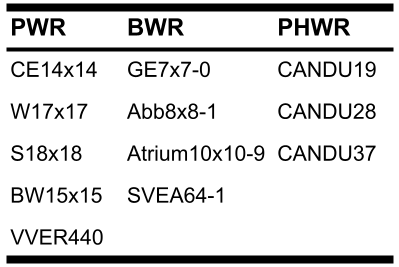
\includegraphics[width=0.5\linewidth]{./chapters/exp1/trainset4_Orxtrs.png}
    \caption{\gls{ORIGEN} designations for reactor technologies and fuel assembly design.}
    \label{tbl:rxtrtype}
    \vspace*{5mm}
  \end{subtable}
  \begin{subtable}{\linewidth}
    \centering
    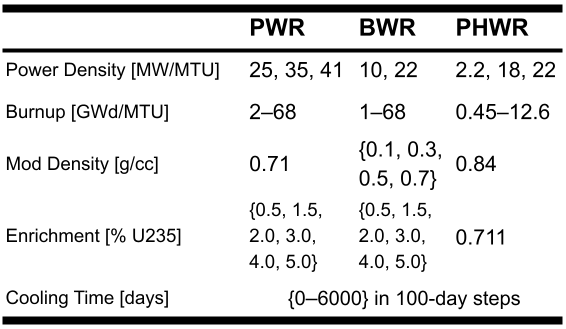
\includegraphics[width=0.75\linewidth]{./chapters/exp1/trainset4_inputs.png}
    \caption{Simulation parameters for \gls{ORIGEN} input files.}
    \label{tbl:rxtrparam}
  \end{subtable}%
  \caption{Training set database design using the \gls{SFCOMPO} database as guidance. \cite{sfcompo}}
  \label{tbl:train}
\end{table}

The design of the training set is dependent on a number of factors.  First, it
must have a sufficient number of burnup sets and time since irradiation steps
to provide robust prediction. This is decided upon by maximizing the steps for
both parameters, while balancing the computational limitations of a large
training set. Through previous experience, an approximate limit would be around
$1e6$ database entries for the specific calculations in this work and employing
reasonable computational limitations.

Secondly, the training set must represent what exists in the real world. This
was accomplished by studying the spread of parameters in the \gls{SFCOMPO}
database \cite{sfcompo}.  To ensure this, a variety of reactor types and
assembly designs were included, listed in Table \ref{tbl:rxtrtype}. Table
\ref{tbl:rxtrparam} lists the rest of the simulation inputs. These include not
only the labels of prediction interest, \gls{U235} enrichment, burnup, and time
since irradiation, but also other important simulation input parameters such as
the reactor power density and the moderator density.  (Water is both the
moderator and coolant in all simulated reactor types.)

\begin{figure}[!hbt]
  \makebox[\textwidth][c]{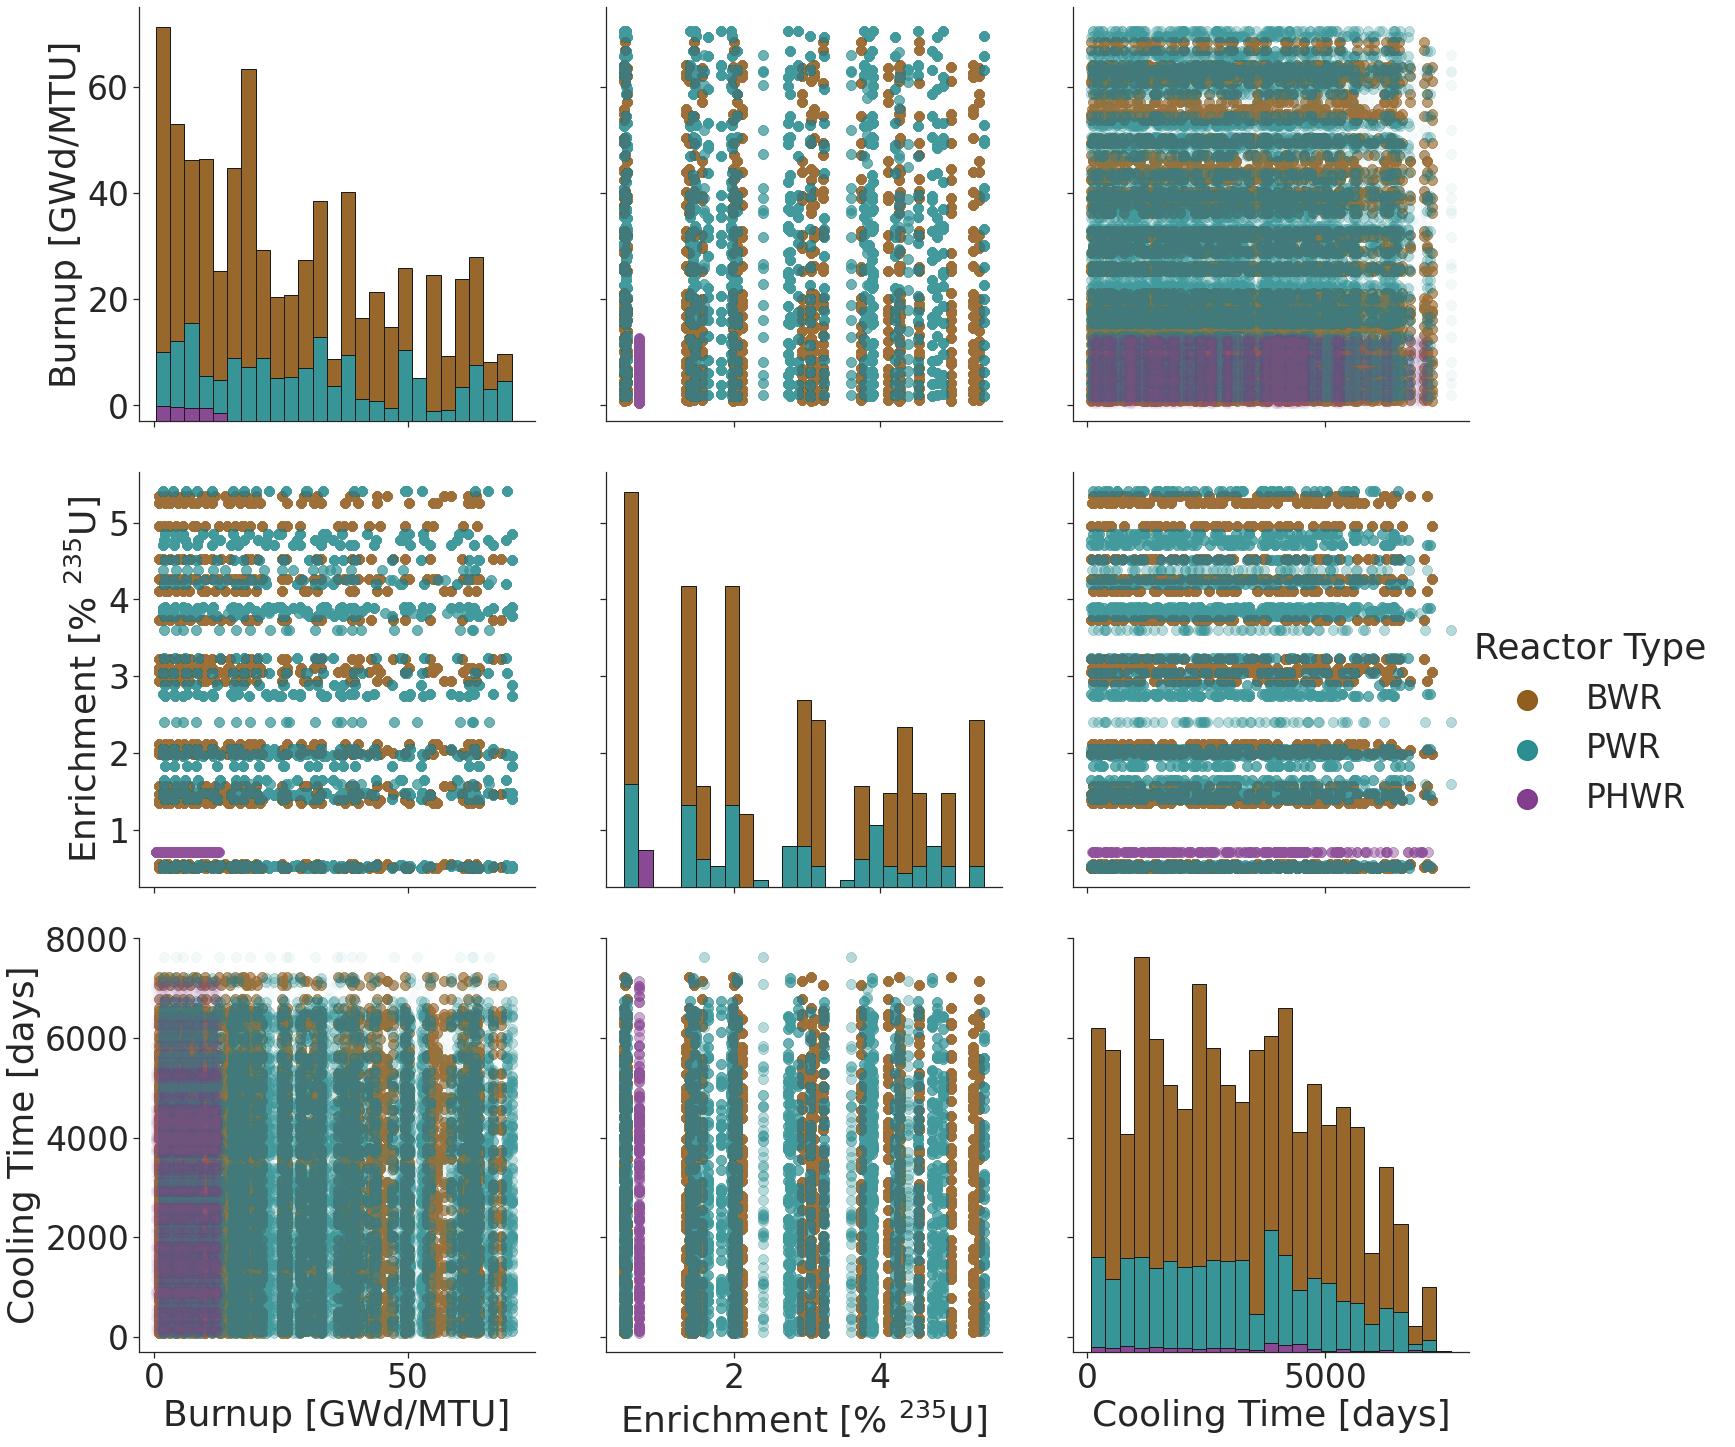
\includegraphics[width=\linewidth]{./chapters/exp1/histogram_scatter_trainset_viz.png}}
  \caption{A combination of histograms and scatter plots to visualize the 
           distribution of prediction labels in the training set.}
  \label{fig:trainhist}
  \todo[inline]{fix the histogram figure, this is a placeholder}
\end{figure}

The third factor influencing database design is ensuring ideal \gls{ML}
algorithm performance.  As mentioned in Section \ref{sec:errs}, many algorithms
are developed with the assumption that the training set will be
\acrfull{i.i.d.}.  This is important so that the model does not overvalue or
overfit a certain area in the training space. With the training set design,
there are predetermined values for enrichment, burnup, and time since
irradiation.  While there are $21-28$ burnup steps (depending on the reactor
type) and 61 cooling time steps, there are only 6 values for enrichment. This
creates the risk that the algorithm will end up being unable to generalize
outside of those discrete values. Therefore, the burnup steps and time steps
are perturbed randomly in a range that is $\pm10\%$ and $\pm30\%$ from the
originally defined values, respectively.  The enrichment also gets perturbed by
$\pm10\%$, and not more because the cross-section libraries in \gls{ORIGEN-ARP}
are pre-calculated for those enrichment values, so deviating too far from them
would result in inaccurate \gls{SNF} simulations. The power densities and
moderator densities were kept at the values defined in Table
\ref{tbl:rxtrparam}.  The resulting training set is $450240$ (or $4.5e5$)
entries.  Figure \ref{fig:trainhist} visualizes the somewhat even distribution
of the burnup and cooling time parameters, and shows the lack of even
distribution of the enrichment parameter through a combination of scatter plots
and histograms.  Note that there are many more \gls{BWR}s present in the
histograms because of the multiple moderator densities simulated (see Table
\ref{tbl:rxtrparam})

\subsection{Training Set Features}
\label{sec:snffeats}

The other design decision regarding the training set is related to
which nuclides to track, i.e., the features.  For this experiment, nuclide
masses are necessary, and the most common measurements in \gls{SFCOMPO} guide
the list of nuclides tracked.  

The set of training features of 29 nuclide masses listed in Table
\ref{tbl:nucmass} was designed with the following reasons in mind.  First, the
units in mass is to represent the scenario of "perfect knowledge", where a full
assay is done via mass spectrometry techniques.  Second, this is to have the
training set units convertable to those present in the external, real-world
test set: the \gls{SFCOMPO} database.  The \gls{ORIGEN} simulations output the
nuclide masses in $grams$, and they are converted to the units of
\textit{milligrams per gram of initial uranium}, $mg/gU_i$, when the models are
externally tested against \gls{SFCOMPO}. Lastly, the 29 nuclides chosen were
based on the presence of measurements in \gls{SFCOMPO}, where these were
present in at least 100 of the samples in the database.  The external test set
is described in more detail in Section \ref{sec:sfcompo}.

\begin{table}[!htb]
  \centering
  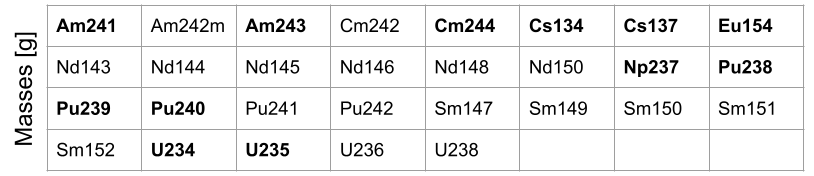
\includegraphics[width=\linewidth]{./chapters/exp1/nucmass_feats.png}
  \caption{Set of features saved for the first experiment, nuclide masses 
           measured in $grams$. The bold nuclide masses overlap with the 
           nuclides in \ref{tbl:nucacts}.}
  \label{tbl:nucmass}
\end{table}



\subsection{Statistical Learning for Models}
\label{sec:statmodel}

\begin{figure}[H]
  \centering
  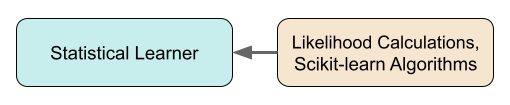
\includegraphics[width=0.7\linewidth]{./chapters/exp2/methodology2_3.png}
  \caption[Third portion of the flowchart from Figure \ref{fig:method2}]
          {Third portion of the flowchart from Figure \ref{fig:method2} being 
           described in this section.}
\end{figure}

The chosen algorithms (\textit{k}-nearest neighbors, decision trees, and
\gls{MLL} calculations) are introduced in Section \ref{sec:algs} and their
implementation details are in Section \ref{sec:statmodel1}.  This section will
therefore only cover the implementation differences from the previous work.
The \gls{MLL} calculations are implemented identically to Chapter
\ref{ch:exp1}.  However, the scikit-learn algorithms in this experiment did
undergo a new round of hyperparameter optimization.

The full list of 22 training sets that undergo training and prediction are as
follows: 
\begin{itemize}
  \item 1 set of nuclide masses (29 nuclide masses from Chapter \ref{ch:exp1})
  \item 3 sets of nuclide activities
    \begin{itemize}
      \item 32 nuclide activities (full knowledge scenario for all nuclides, 
            whether or not they are present in a quantity able to be detected)
      \item 12 nuclide activities (full knowledge for long energy windows list)
      \item 7 nuclide activities (full knowledge for short energy windows list)
    \end{itemize}
  \item 18 detector-based processed spectra sets
    \begin{itemize}
      \item Auto energy windows lists applied to six detectors (lab-based 
            \gls{HPGe}, portable \gls{HPGe}, \gls{CZT}, \gls{SrI2}, \gls{LaBr3}, 
            \gls{NaI})
      \item Short energy windows lists applied to six detectors above
      \item Long energy windows lists applied to six detectors above
    \end{itemize}
\end{itemize}

\begin{table}[!htb]
  \centering
  \begin{tabular}{@{}llcll@{}}
    \toprule
    \textbf{\begin{tabular}[c]{@{}l@{}}Training Set\\ Description\end{tabular}} &
    \textbf{\begin{tabular}[c]{@{}l@{}}Prediction\\ Parameter\end{tabular}} &
    \textbf{\begin{tabular}[c]{@{}l@{}}\textit{k} \\ (N neighbors)\end{tabular}} &
    \textbf{\begin{tabular}[c]{@{}l@{}}Max \\ Depth\end{tabular}} &
    \textbf{\begin{tabular}[c]{@{}l@{}}Max \\ Features\end{tabular}} \\ 
    \toprule
    \multirow{4}{*}{\begin{tabular}[c]
    {@{}l@{}}29 \\ Nuclide\\ Masses\end{tabular}}          & Reactor Type & 4 & 56 & 29          \\
                                                           & Burnup       & 1 & 77 & 29          \\
                                                           & Enrichment   & 1 & 73 & 29          \\
                                                           & Cooling Time & 2 & 45 & 29          \\ 
                                                           \hline
    \multirow{4}{*}{\begin{tabular}[c]
    {@{}l@{}}32\\ Nuclide\\ Activities\end{tabular}}       & Reactor Type & 1 & 41 & 32          \\
                                                           & Burnup       & 1 & 49 & 32          \\
                                                           & Enrichment   & 1 & 67 & 32          \\
                                                           & Cooling Time & 7 & 56 & 32          \\
                                                           \hline
    \multirow{4}{*}{\begin{tabular}[c]
    {@{}l@{}}7 or 12\\ Nuclide \\ Activities\end{tabular}} & Reactor Type & 1 & 67 & 7 or 12     \\
                                                           & Burnup       & 1 & 78 & 7 or 12     \\
                                                           & Enrichment   & 1 & 60 & 7 or 12     \\
                                                           & Cooling Time & 4 & 68 & 7 or 12     \\
                                                           \hline
    \multirow{4}{*}{\begin{tabular}[c]
    {@{}l@{}}Energy \\ Windows:\\ Short\end{tabular}}      & Reactor Type & 1 & 62 & 42          \\
                                                           & Burnup       & 1 & 62 & 42          \\
                                                           & Enrichment   & 4 & 64 & 42          \\
                                                           & Cooling Time & 2 & 54 & 42          \\
                                                           \hline
    \multirow{4}{*}{\begin{tabular}[c]
    {@{}l@{}}Energy \\ Windows:\\ Long\end{tabular}}       & Reactor Type & 4 & 62 & 151         \\
                                                           & Burnup       & 1 & 51 & 151         \\
                                                           & Enrichment   & 5 & 73 & 151         \\
                                                           & Cooling Time & 2 & 64 & 151         \\
                                                           \hline
    \multirow{4}{*}{\begin{tabular}[c]
    {@{}l@{}}Energy \\ Windows:\\ Auto\end{tabular}}       & Reactor Type & 2 & 61 & None or 150 \\
                                                           & Burnup       & 1 & 52 & None or 150 \\
                                                           & Enrichment   & 4 & 67 & None or 150 \\
                                                           & Cooling Time & 2 & 58 & None or 150 \\ 
    \bottomrule 
  \end{tabular}
  \caption[Optimized algorithm hyperparameters for all training sets in second 
           experiment]
          {Optimized algorithm hyperparameters; the energy lists took all 
           detectors into account.}
  \label{tbl:exp2hypparam}
\end{table}

Table \ref{tbl:exp2hypparam} lists the hyperparameter optimization results for
the 22 training sets. Because the 29 nuclide mass training set is included in
this chapter for comparison, its optimization results are also listed here.
The number of features for decision trees are not limited because the test runs
for optimization provided highly variable results. The only case where this is
not true is with the auto energy windows list for the lab-based \gls{HPGe} with
a length of 206; the maximum features for this one case are limited to 150.
Instead, optimization was carried out only on the maximum depth for decision
trees with keeping the full length of features.  This is an area that could
undergo deeper exploration than what occurs in this work, since the training
sets with large feature sets can become overfit.

The optimization took place in two rounds, where the first round had a coarser
grid of \textit{k} for \textit{k}-nearest neighbors and maximum depth for
decision trees and the second round had a finer grid of parameters. The 7 \& 12
nuclide activity training sets were optimized separately but contain averages
of the two results for the maximum depth, and the higher value of \textit{k}
when the two did not match. The \textit{k} and maximum depths were averaged
across all six detectors for each energy window list length (short, long, and
auto).  There were fairly consistent results from the short and long lists, but
the variable length of the auto-generated energy windows lists (in Table
\ref{tbl:enwindows}) gave a wider range of ideal hyperparameters.



\subsection{Validation}
\label{sec:valid}
To obtain reliable models, one must both choose or create a training set
carefully and study the impact of various algorithm parameters on the error.
Although the title of this section suggests final steps of confirming a model's
usefulness for predictions, what follows is more of a troubleshooting exercise. 
In practice, these analyses are used for both purposes.

Machine learning algorithms are heavily dependent on the inputs and parameters
given to them, such as training set sizes, regularization, learning rates, etc.
From the results shown in Section \ref{sec:statmodel}, it is clear there is
room for improvement.  Diagnostic plots show the errors of the predicted
burnup values to the actual burnup values with respect to some variable on the
\textit{x}-axis.  As previously introduced in Section \ref{sec:optvalid}, the
errors are compared to the training error to understand the generalization
strength with respect to training set size (learning curves) and the algorithm
parameters governing model complexity (validation curves). 

In addition to machine learning best practices, another layer of comparison is
added here.  Because it is difficult to ensure consistently representative
testing data, the accuracy of a learned model should not depend on only one
testing set.  The learned model's accuracy is better estimated by using a
validation set, or even better, \textit{k}-fold cross-validation, introduced in
Section \ref{sec:selectass}. This work includes both the testing error (using
the testing set described in Section \ref{sec:training}) and cross-validation
error. The predetermined testing set will allow for comparison against the
previous work it was obtained from \cite{dayman_feasibility_2013}, but it is
assumed that cross-validation will provide a better indication of model
performance.

\begin{figure}[!htb]
    \centering
    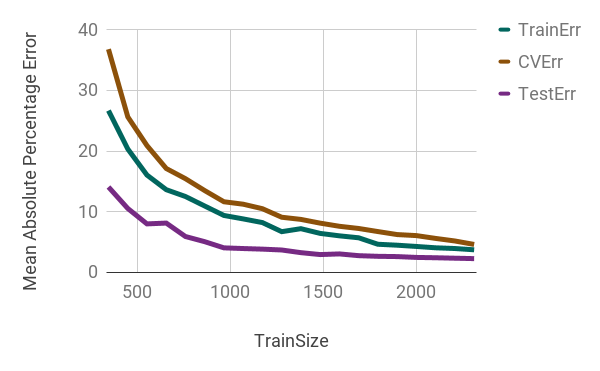
\includegraphics[width=\linewidth]{./chapters/demo_method/lc1.png}
    \caption{Learning curve for burnup prediction, $\gamma = 0.001$}
    \label{fig:lc1}
\end{figure}

The learning curves are obtained as follows, shown in Figure \ref{fig:lc1}.
For a given (randomly chosen) training set size between 15 and 100\% of the
total data set, training and prediction rounds were performed for each. The
testing error scenario performs this \textit{k} times and averages those
results.  This is equivalent to the \textit{k} in \textit{k}-fold
cross-validation to provide some semblance of equivalent statistics.  The
cross-validation error scenario has no need for averaging because it is
performed automatically. In both cases, the learning curves do not provide a
clear picture of over- or undertraining upon first glance.

\begin{figure}[!htb]
    \centering
    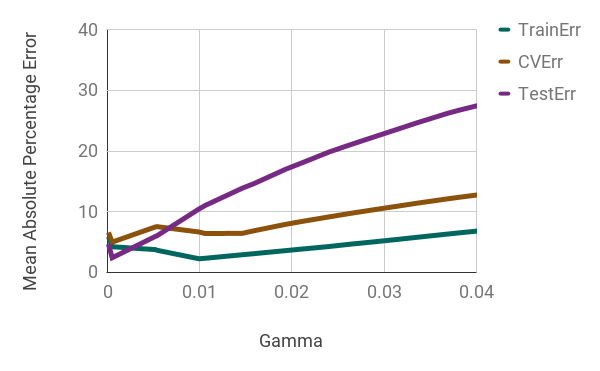
\includegraphics[width=\linewidth]{./chapters/demo_method/vc1.png}
    \caption{Validation curve for burnup prediction, $TrainSize = 2313$}
    \label{fig:vc1}
\end{figure}

The validation curves are obtained as follows, shown in Figure \ref{fig:vc1}.
The $\gamma$ parameter in \gls{SVR}, which influences model complexity, was
varied from $10^{-4}$ to $10^{-1}$. Training and prediction rounds were
performed for different $\gamma$ values in this range.  Again, the testing and
cross-validation errors are both used as described above. As with Figure
\ref{fig:lc1}, determining the robustness to over- or undertraining is
difficult here although there is possibly a minimum at $\gamma = 0.001$.

Although there is no example behavior of Figure \ref{fig:lc1}'s peculiar
learning curve in Figure \ref{fig:learning}, the curve mimics the squared bias
curve from Figure \ref{fig:bvtradeoff}. This indicates that the bias in the
model is much higher than the variance.  Next, the testing error is lower than
the training error; this should never be the case, and indicates an issue with
the systematically chosen testing set.  While the cross-validation error is
correctly higher than the training error, it follows along in parallel,
producing no information on model fitness other than confirming a very high
bias.  It is presumed this is not the fault of the algorithms, but the training
set itself.  It is likely covering too small of a range of the simulation
space.

Additionally, Figure \ref{fig:vc1}'s validation curve shows the testing error
dropping below the training error for extremely small $\gamma$, around where a
minimum might be.  Since the model suffers from high bias, no amount of model
complexity can be optimized. The resolution to the underfitting is discussed in
Section \ref{sec:prep}.




\section{Experimental Demonstration}
\label{sec:expdemo}
\todo{redo outline/section titles here later}

The first steps of this work include a loose replication of the previously
mentioned work studying the effect of information reduction on predictions
\cite{dayman_feasibility_2013}, and comparing this to the more complex algorithm chosen.
This helped to establish some baseline expectations of reactor
parameter prediction and how the different algorithms perform. 

First discussed are the preliminary results in Section \ref{sec:results}, which
indicated the models were severely underfitted. Following that, the next step
was to provide a larger, more diverse training set to the algorithms so they
could predict better when faced with new instances. This is shown in Section
\ref{sec:newtrain}. 

\todo{Not sure about last section yet}

\subsection{Results}
\label{sec:results}

Some kind of results section here with validation, or just eval and conclusions.

\subsection{Expanding the Training Set Space}
\label{sec:newtrain}

This is what I did based on the results, and here are more results and validation.
Dayman training/test set -> sfcompo-like sims and testing set

\subsection{Comparing Different Models}
\label{sec:compare}

Will I have prob density for prelim? Prob not?
